
\section{Signals and properties}

\subsection{Properties of analog signals}

\paragraph{Analog signal} We define a signal is this course as a function of
time or space. For instance $x:\R\rightarrow\dbC$ is a complex 1D signal of time
$t\in\dbR$. $x:\R^2\rightarrow\dbR$ is a 2D image of space $\p\in\dbR^2$.

\paragraph{Causality}\index{Causal signal}
A signal $x(t)$ is causal if 
$$ x(t)=0,\quad \forall x<0 $$

Example: $x(t)= \begin{cases}
0& \text{for } t<0\\
\sin(t)\exp\left(-\frac{t^2}{2}\right) & \text{for } t\geq 0
\end{cases}$

\paragraph{Periodicity}\index{Periodic signal} 
A signal $x(t)$ is periodic of period $T_0$ is
$$x(t-kT_0)=x(t),  \forall t\in\mathbb{R}, \forall k\in\mathbb{N}$$      


Example: $x(t)= %\begin{cases}
 % \exp(-\frac{(t-1)^2}{2})&  0<t<T\\
  \exp\left(-\frac{(t-kT_0-1)^2}{2}\right)  \text{ for }kT_0<t<(k+1)T_0,\quad
  \forall k\in\mathbb{N}$
  
\begin{figure}[t]
    \centering
    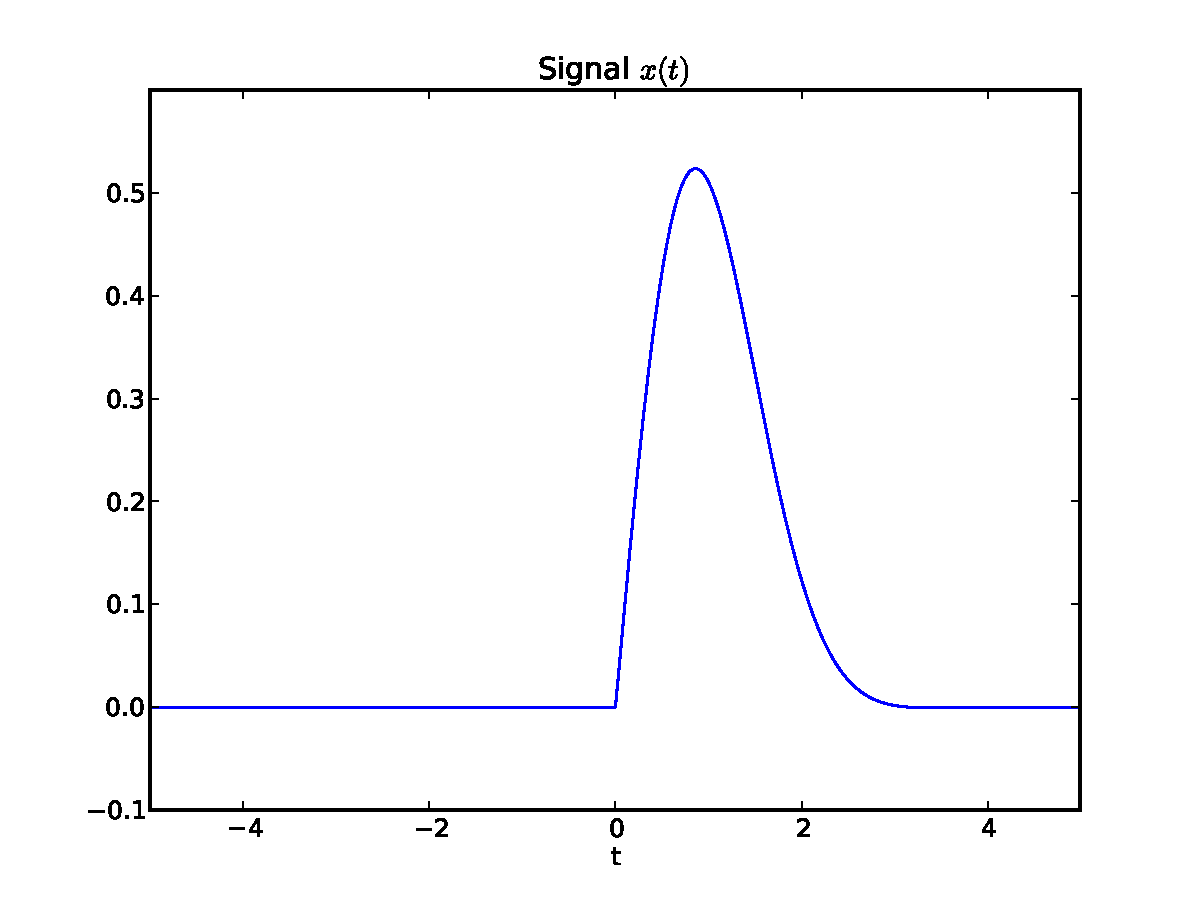
\includegraphics[width=.45\linewidth]{imgs/sig_conv/sig_causal.pdf}
    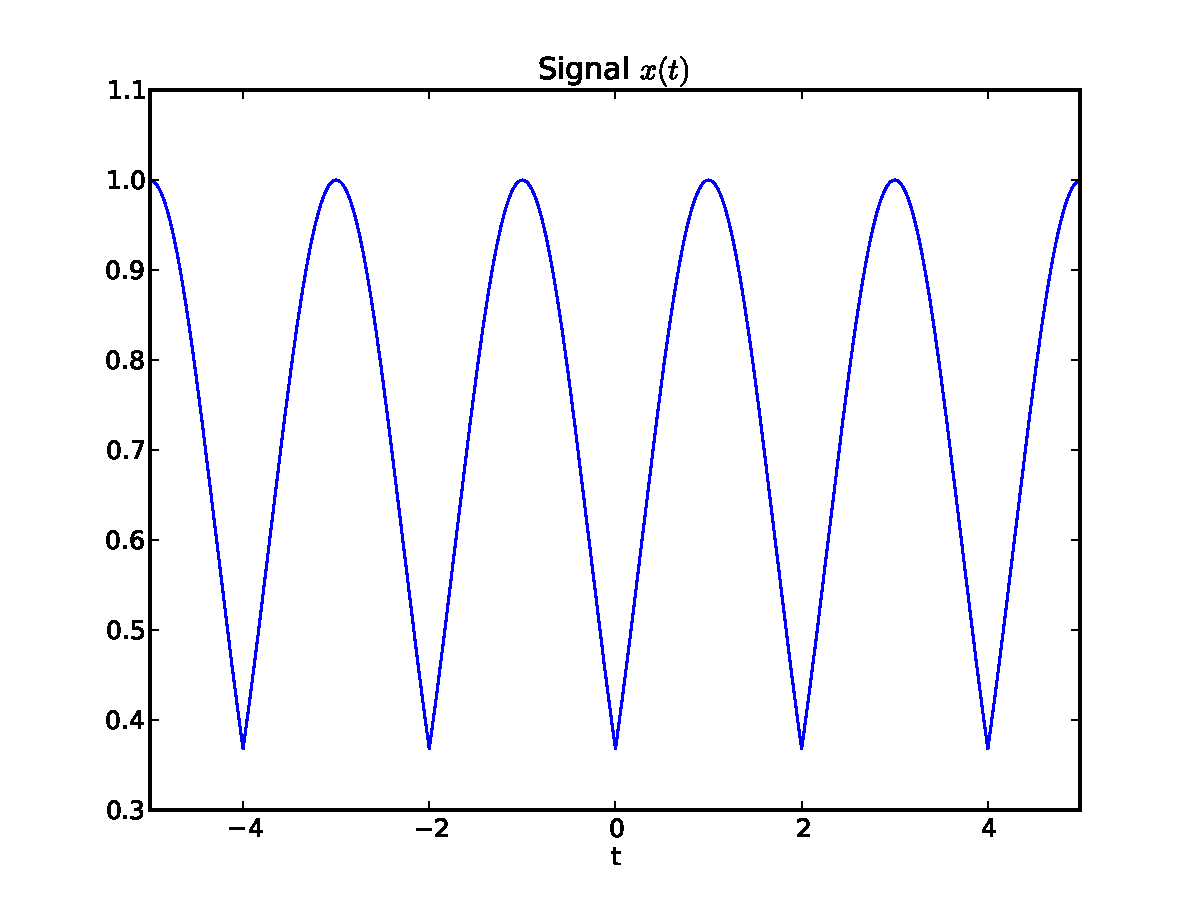
\includegraphics[width=.45\linewidth]{imgs/sig_conv/sig_per.pdf}
    \caption{Examples of Causal signal (left) and periodic signal (right).}
    \label{fig:ex_causal_per}
\end{figure}



\paragraph{Signal in $L_p$ space}\index{$L_p$ space}
$L_p(S)$ is the set of functions whose absolute value to the power of $p$
has a finite integral or equivalently that
\begin{equation}
  \|x\|_p=\int_S |x(t)|^p dt < \infty
  \label{eq:lp_space}
\end{equation}
\begin{itemize}
  \item $L_1(\dbR)$ is the set of absolute integrable functions
  \item $L_2(\dbR)$ is the set of quadratically integrable functions (finite energy)
  \item $L_\infty(\dbR)$ is the set of bounded functions
\end{itemize}

\paragraph{Instantaneous power}\index{Power}
The instantaneous power of signal $x(t)$ 
\begin{equation}
  \label{eq:puissinst}
  p_x(t)=|x(t)|^2
\end{equation}
 Unit :  Watt (W).


 \begin{block}{Energy of a signal}\index{Energy}
  We define the energy of a signal $x(t)$ as :
\begin{equation}
\label{eq:enerfinie}
E=\pause \int_{-\infty}^{+\infty}|x(t)|^2dt
\end{equation}
the signal is said to be of finite energy if $E<\infty$ ($\|x\|_2<\infty$ means $x\in L_2(\dbR)$).

Unit: Joule, Calorie or Watt-hour (J, Cal ou Wh, 1 calorie = 4.2 J).
\end{block}

\begin{block}{Average power of a signal}
  
  The average power of a signal is defined as
   \begin{equation}
     \label{eq:puissance}
    P_m= \pause\lim_{T\rightarrow\infty} \frac{1}{T}\int_{-\frac{T}{2}}^{+\frac{T}{2}}|x(t)|^2dt
   \end{equation}
   \begin{itemize}
   \item For a periodic signal, the average power can be computed on a unique period.
   \item Power is homogeneous to an energy divided by time.
   \item $P_{RMS}=\sqrt{P_m}$ is called the Root Mean Square power ("valeur efficace" in french).
   \item A finite energy signal has a n average power $P_m=0$.
   \item  Unit :  Watt (W).
   \end{itemize}
   
     \end{block}


     \begin{block}{Additive noise}
      Additive noise is a kind of noise that is added to the signal of interest.
  $$y(t)=x(t)+b(t)$$
  $y(t)$ is the observed signal, $x(t)$ the signal of interest and
  $b(t)$ is the noise.
    \end{block}

    \begin{block}{Signal-to-Noise ratio (SNR)} \index{SNR}\index{Signal-to-Noise ratio}
      The Signal to Noise Ratio is defined as:
  \begin{equation}
    \label{eq:rsb}
    SNR=\frac{P_S}{P_N} \quad \text{ ou } \quad SNR(dB)=10\log_{10}(SNR)
  \end{equation}
  where $P_S$ is the power of the signal and $P_N$ the power of the noise.
  \begin{itemize}
  \item An Analog-to-Digital conversion process should have the best possible SNR.
  \item The SNR is often used for additive noise models.
  \item Other measures such as Peak Signal to Noise Ratio (PSNR) can be used on specific data (images).
  %\item Le RSB est également appelé SNR pour Signal to Noise Ratio.
  %\item Le Rapport signal sur signal + bruit est également utilisé.
  %$$ R_{S/S+B}=\frac{P_S}{P_{S+B}}$$
  \item One of the objective of filtering is to get a better SNR when the signal and the noise have different frequency contents..
  \end{itemize}
    \end{block}





\subsection{Common signals}
\label{sec:common_sig}


\begin{block}{Heaviside function}
  \begin{equation}
\label{eq:heaviside}
\Gamma(t)=
\begin{cases}
  0& \text{if } t<0\\
  1/2& \text{if } t=0\\
  1 & \text{if } t>0
\end{cases}
\end{equation}
%Exemple: On allume une ampoule.
Also known as the step function. \index{Function!Heaviside}
\end{block}

\begin{block}{Rectangular function}\index{Function!Rectangular}
  \begin{equation}
   \Pi_T (t)=
   \begin{cases}
     1/T& \text{if } |t|< T/2\\
     1/2T& \text{if } |t|= T/2\\
     0& \text{else}
   \end{cases}
   \label{eq:rectangular}
 \end{equation}
 %\vspace{-.5cm}
 \begin{itemize}
 \item $\Pi(t)=\frac{1}{T}(\Gamma(t-\frac{T}{2})-\Gamma(t+\frac{T}{2}))$.
 \item Finite energy signal (finite support).
 \end{itemize}
   \end{block}


   \begin{block}{Complex exponential }\index{Function!Complex exponential}
    let $e_z(t)$ be the following function $\dbR \rightarrow \dbC$
 \begin{equation}
   \label{eq:expcomplexe}
   e_z(t)=\exp(zt)
 \end{equation}
 where $z$ is a complex number.
 When $z=\tau+wi$ the, 
 \begin{equation*}
   \label{eq:expcomplexe2}
   e_z(t)=(\cos(wt)+i\sin(wt))\exp(\tau t)
 \end{equation*}
 %\vspace{5mm}
 
 
 Special cases:
 \begin{itemize}
 \item $z=\tau$ real, then we recover the classical exponential.
 $$e_z(t)=\exp(\tau t)$$
 
 \item $z=wi$ imaginary then
 $$e_z(t)=\cos(wt)+i\sin(wt) $$
 
 % \item $z=\tau+wi$ quelconque alors
 %   $x(t)=(\cos(w*t)+i*\sin(w*t))\exp(\tau t)$
 \end{itemize}
   \end{block}

\begin{figure}[ht]
  \centering
  \begin{tabular}{|c|ccc|}\hline
    $\tau \backslash w$ & $-2$ & $0$ & $2$ \\\hline
   \raisebox{9mm}{$-0.5$} 
    & 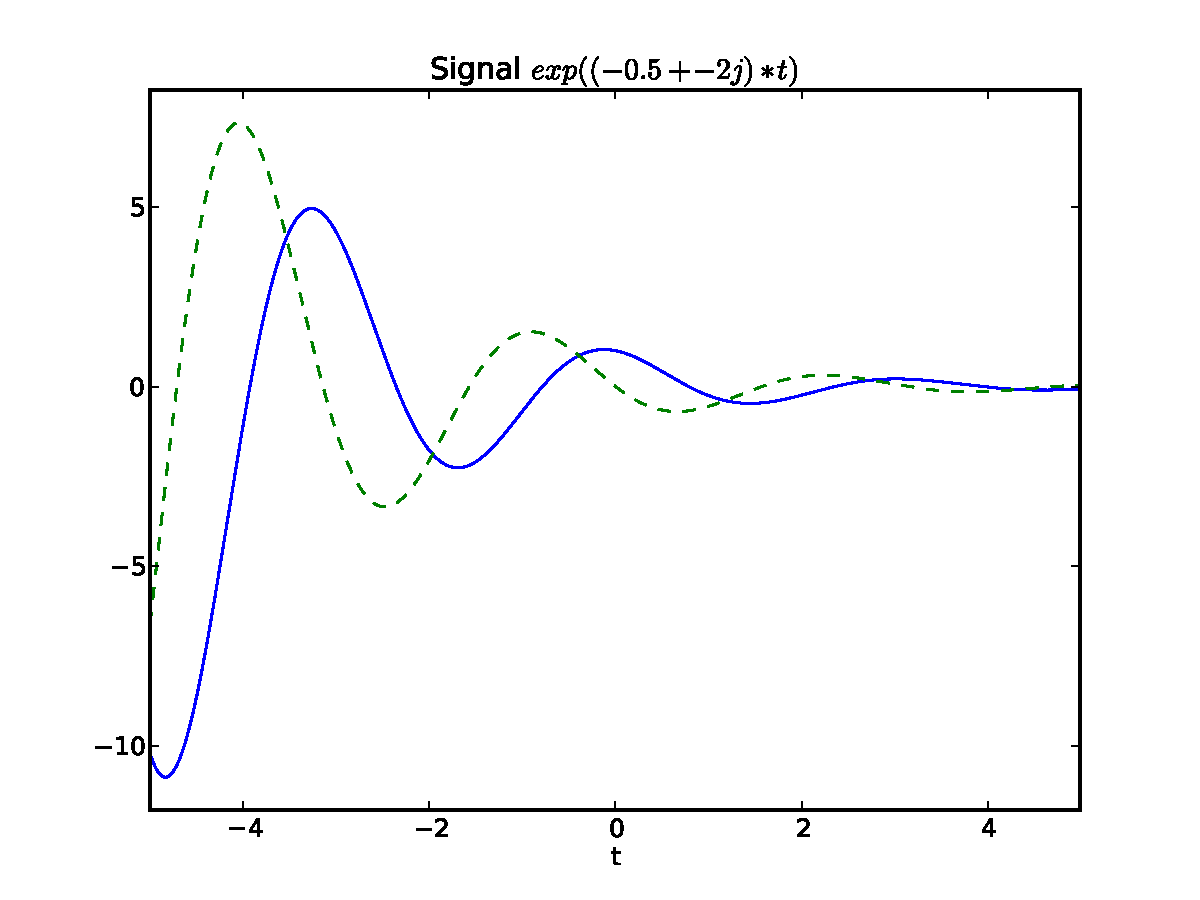
\includegraphics[width=.25\linewidth]{imgs/sig_conv/sig_exp-1-1.pdf}
    & 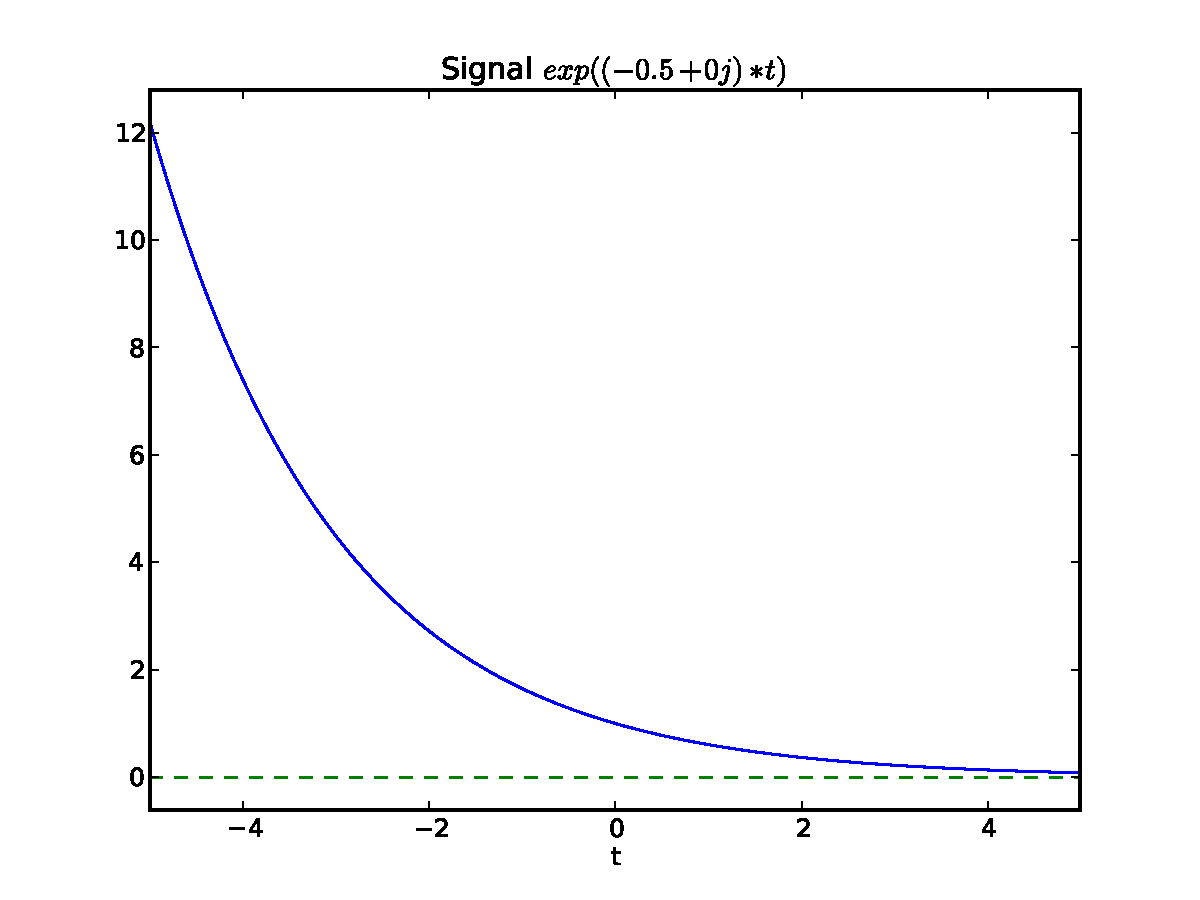
\includegraphics[width=.25\linewidth]{imgs/sig_conv/sig_exp-10.pdf}
    & 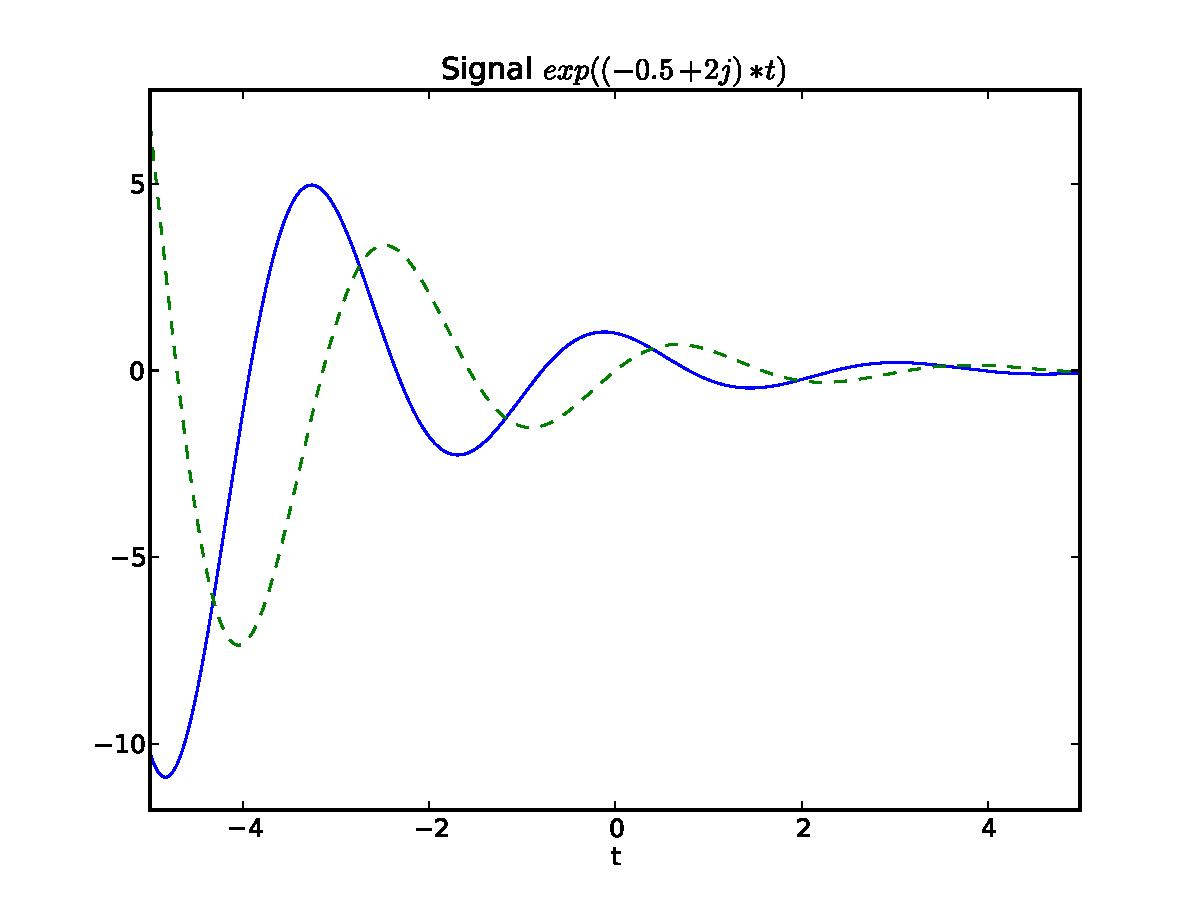
\includegraphics[width=.25\linewidth]{imgs/sig_conv/sig_exp-11.pdf}\\
   \raisebox{9mm}{$0$} 
    & 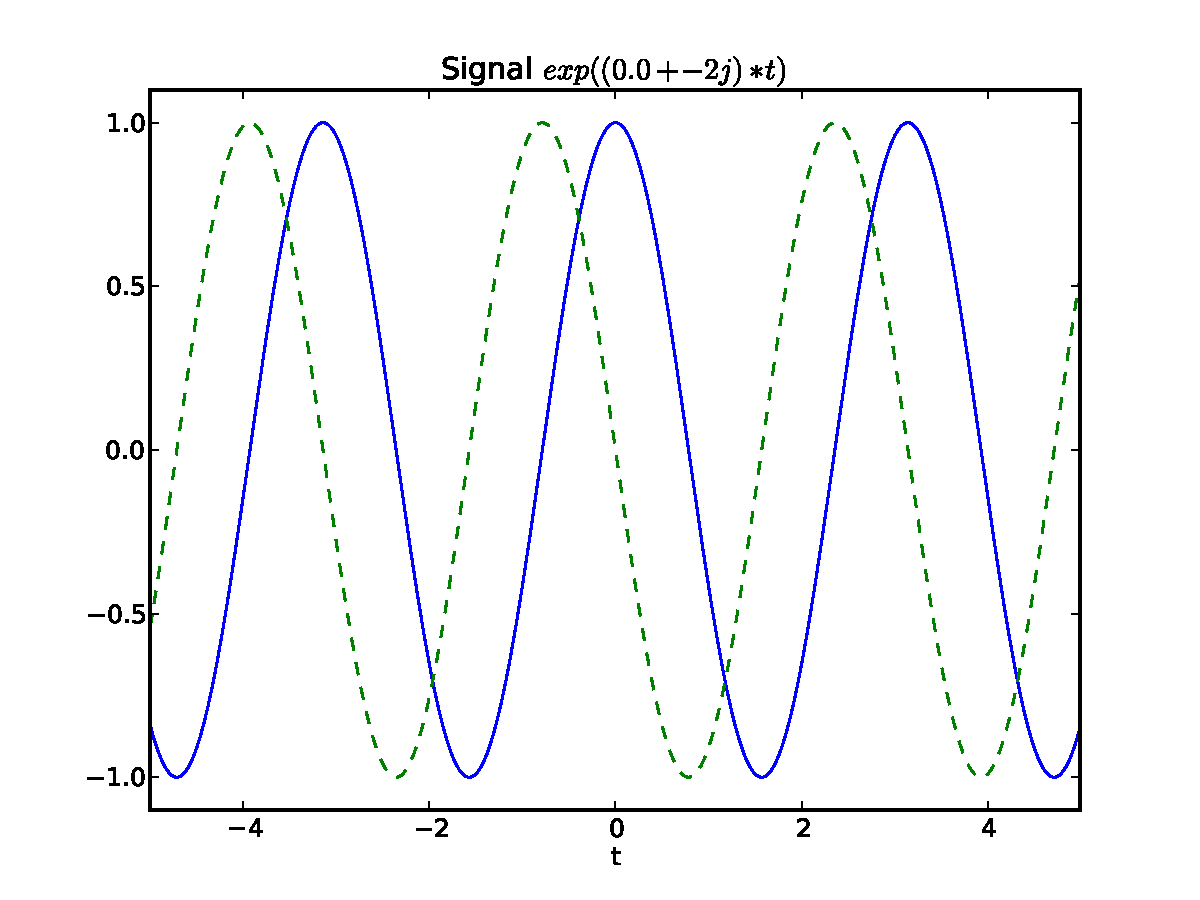
\includegraphics[width=.25\linewidth]{imgs/sig_conv/sig_exp0-1.pdf}
    & 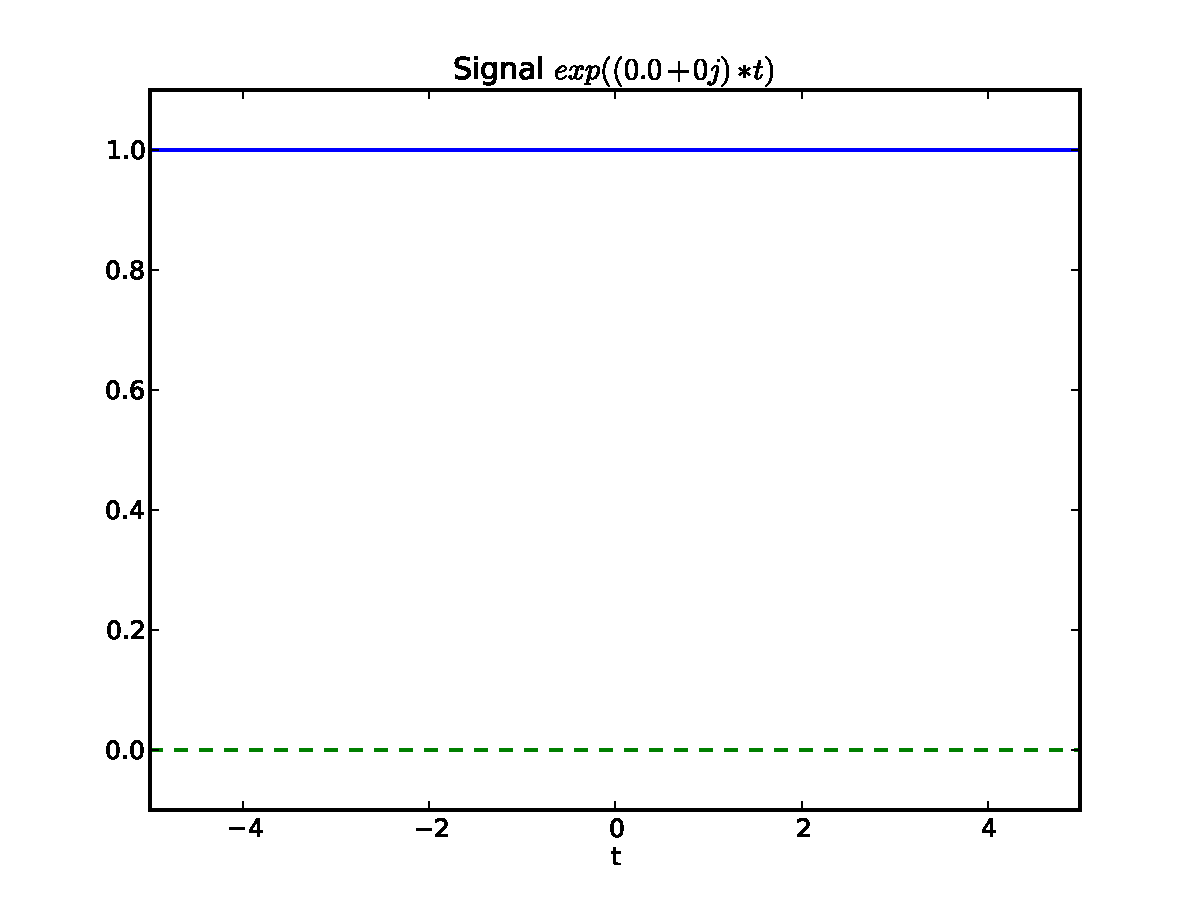
\includegraphics[width=.25\linewidth]{imgs/sig_conv/sig_exp00.pdf}
    & 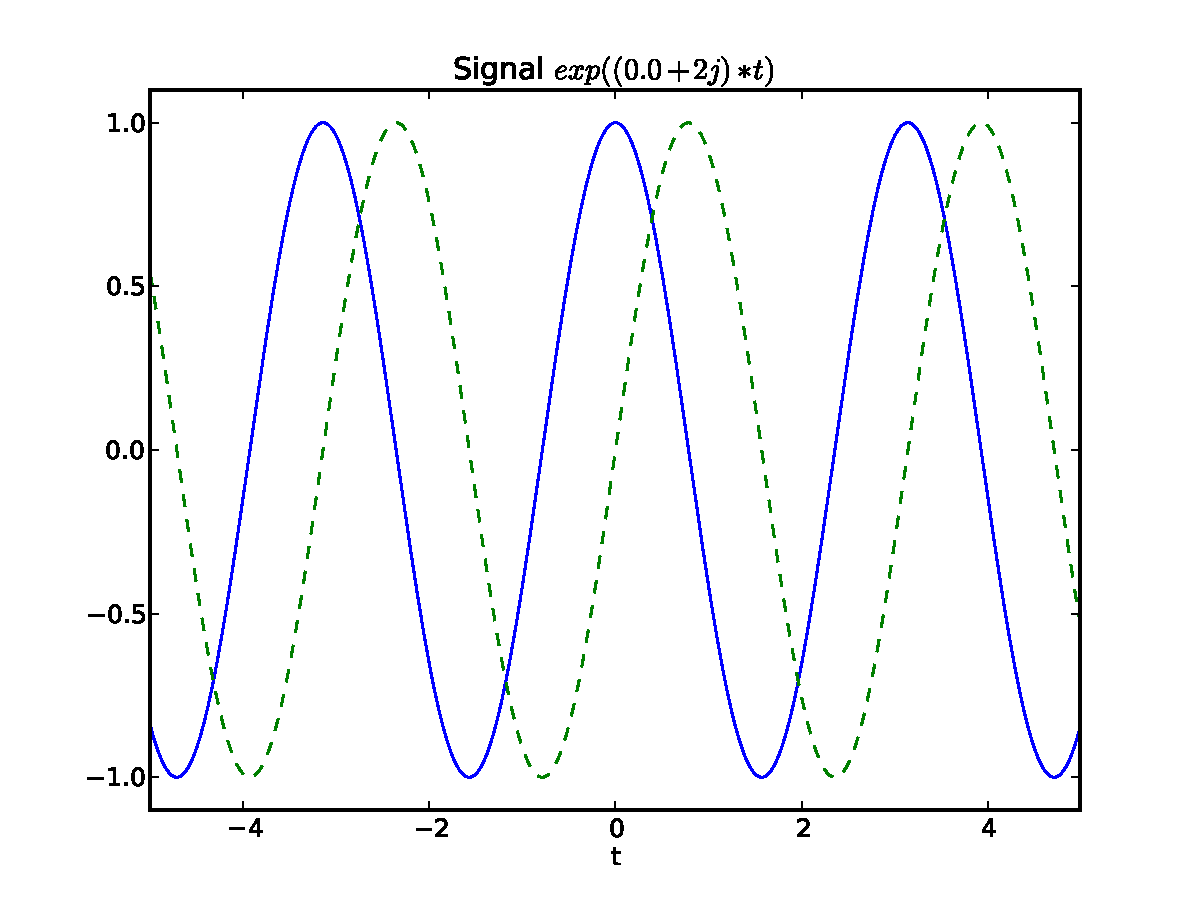
\includegraphics[width=.25\linewidth]{imgs/sig_conv/sig_exp01.pdf}\\
   \raisebox{9mm}{$.5$} 
    & 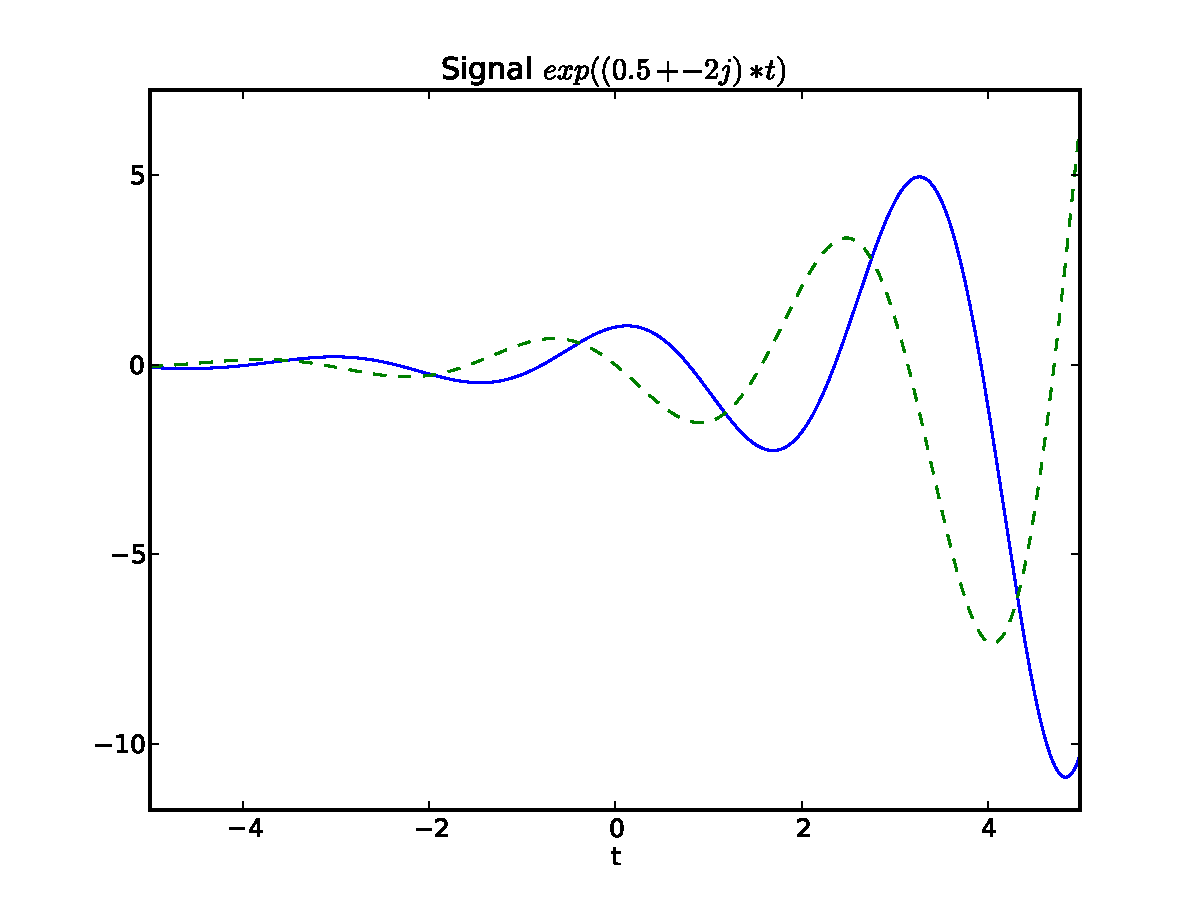
\includegraphics[width=.25\linewidth]{imgs/sig_conv/sig_exp1-1.pdf}
    & 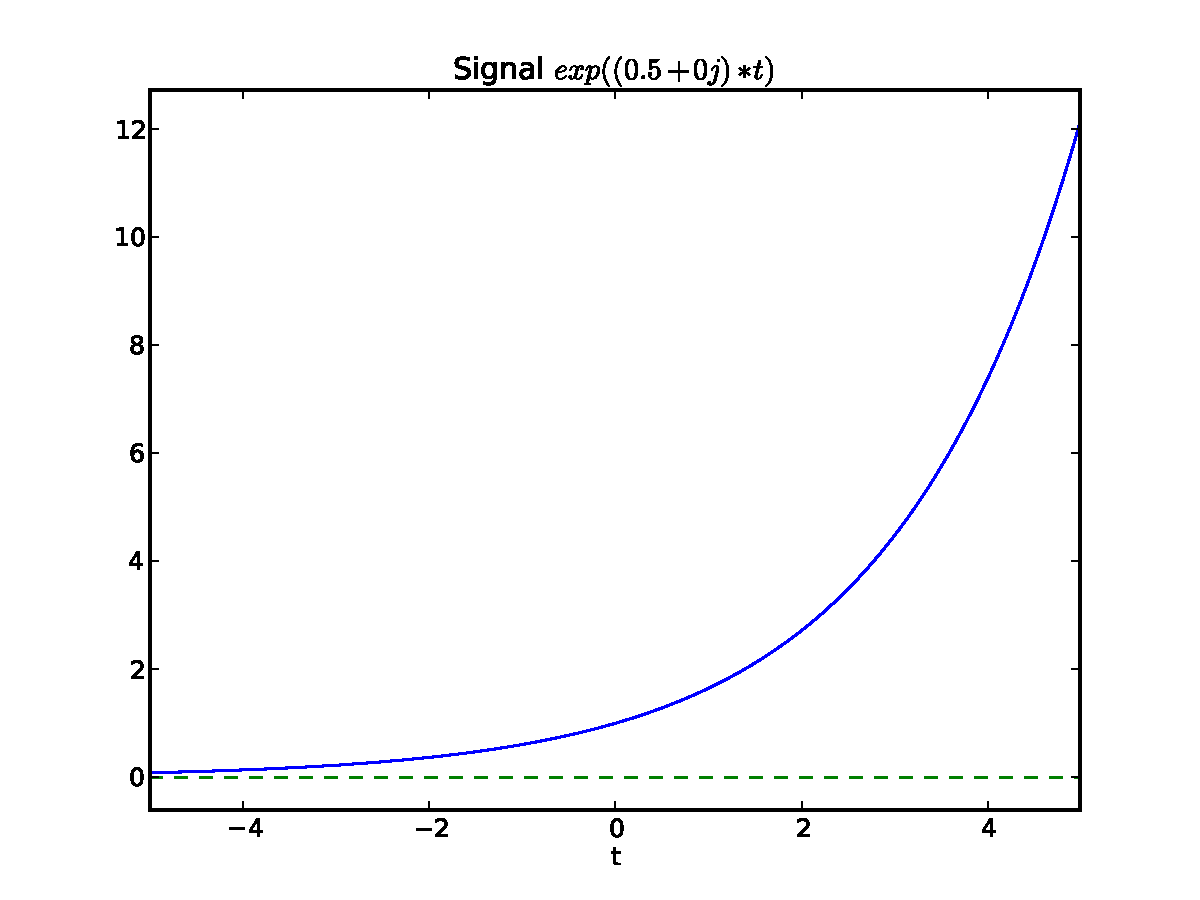
\includegraphics[width=.25\linewidth]{imgs/sig_conv/sig_exp10.pdf}
    & 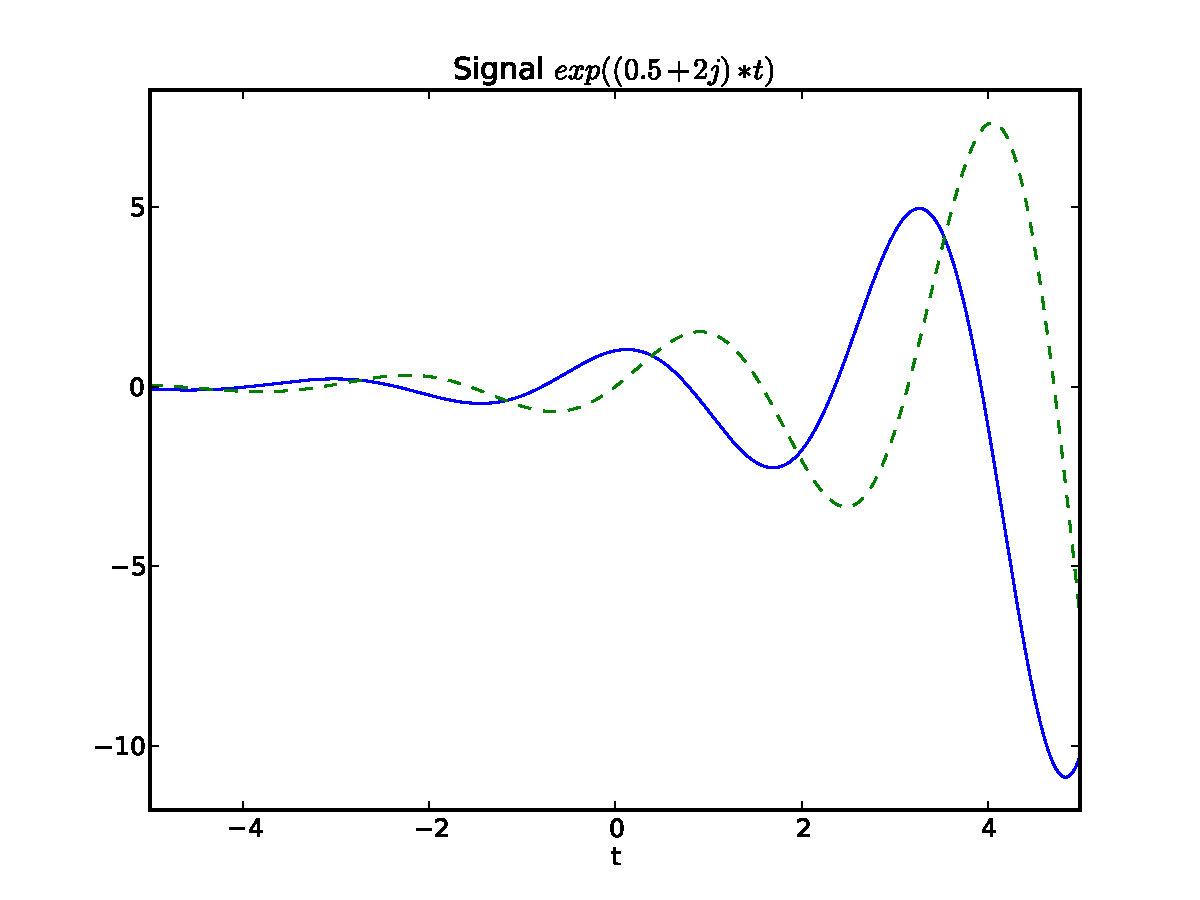
\includegraphics[width=.25\linewidth]{imgs/sig_conv/sig_exp11.pdf}\\
\hline
  \end{tabular}
  \caption{Example of complex exponential for different values of $z$}
  \label{fig:label}
\end{figure}

\subsubsection{Dirac delta}

\index{Dirac delta}
\index{Function!Dirac delta}

\begin{block}{Main properties of Dirac delta}


  \begin{itemize}
    \item Model point mass at $0$.
    \item Value outside $0$ :  $\delta(t)=0, \forall t\neq 0$ 
    %\item Can also be defined as $\lim_{T\rightarrow \infty} \Pi_T(t)$
    \item $\delta$ is a tempered distribution. % (not a function).
    \item Very useful tool in signal processing
   % \item All integrals with $\delta$ will be Lebesgue.
    \item Can be seen as the derivative of the Heavyside function $1_{t\geq 0}(t)$
    \item Integral
    \begin{equation}
      \label{eq:intdirac}
      \int_{-\infty}^{+\infty}\delta(t)dt=1 ,\qquad \int_{-\infty}^{+\infty}x(t)\delta(t)dt=x(0)
    \end{equation}
    \item Dirac and function evaluation for signal $x(t)$ and $t_0\in\R$ :
    %  $$ \delta(t)x(t)=\delta(t)x(0) $$
      $$\delta(t-t_0)x(t)=\delta(t-t_0)x(t_0) $$
   % \item Function evaluation :
    \begin{equation}
      \label{eq:diraceval}
      \langle  x(t) , \delta(t-t_0)\rangle=\int_{-\infty}^{+\infty}x(t)\delta(t-t_0)dt=x(t_0)
    \end{equation}
  
  \end{itemize}
  
  
  \end{block}

  \begin{block}{ Dirac delta definition}

    \begin{itemize}
      \item Let $\phi$ a function supported in $[-1,1]$ of unit mass: $\int_{-\infty}^\infty \phi(u)du=1$ 
      \item  $\phi_T(t)=\frac{1}{T}\phi(\frac{t}{T})$ has support on $[-T,T]$ and unit mass.
      \item We can define the dirac delta $\delta$ as
      $$ \delta(t)=\lim_{T\rightarrow 0} \phi_T(t) $$


    \end{itemize}
    
    
    \end{block}


    \begin{block}{Delta dirac in practice}
      \begin{itemize}
        \item Theoretical object in signal processing (impulse).
        \item Used to model signal sampling for digital signal processing.
        \item Used to model point source  in Astronomy/image processing, point charge in Physics.
        \item Has a bounded discrete variant.
      \end{itemize}
    \end{block}


\frametitle{The dirac comb}\index{Dirac comb}\index{Function!Dirac comb}

\begin{itemize}
  \item The dirac comb is expressed as
  \begin{equation}
    \Sh_T(t)=\sum_{k=-\infty}^\infty \delta(t-kT)
    \label{eq:dirac_comb}
  \end{equation}
  where $\Sh$ is the Cyrilic Sha symbol.
  \item The Fourier Transform of the dirac comb is 
  \begin{equation}
    \mathcal{F}[\Sh_T(t)]=\sum_{k=-\infty}^\infty e^{2i\pi k T f}= \frac{1}{T}\sum_{k=-\infty}^\infty \delta\left(f-\frac{k}{T}\right) =  \frac{1}{T}\Sh_{\frac{1}{T}}(f)
    \label{eq:ft_dirac_comb}
  \end{equation}
  where the second equality comes from the Poisson summation formula.
  \item The dirac comb is used to perform a regular temporal sampling.
  \item Multiplying a signal by the dirac comb corresponds to a convolution by a dirac comb in the Frequency domain (and vice versa).
\end{itemize}
%\end{example}

    \subsection{Discrete time and digital signals}
    \label{sec:}
    

\section{Convolution and filtering}
\label{sec:conv_filtering}

\subsection{Convolution and properties}
\label{sec:}

\index{Convolution}.
\begin{block}{Convolution}
  Let two signals $x(t)$ and $h(t)$. The convolution between the two signals
  is defined as
  \begin{equation}
    x(t)\star h(t) =  \int_{-\infty}^{+\infty}x(\tau)h(t-\tau)d\tau
    \label{eq:convolution}
  \end{equation}\vspace{-5mm}
  \begin{itemize}
    \item Convolution is a bilinear mapping between $x$ and $h$.
    \item It models the relation between the input and the output of a Linear
    Time Invariant system.
    \item If $f\in L_1(\R)$ and $h\in L_p(\R), p\geq1$ then
    $$ \|f\star h\|_p\leq\|f\|_1\|h\|_p $$
    \item The dirac delta $\delta$ is the neutral element for the convolution operator:
\begin{equation}
      \label{eq:dirac_conv}
     x(t)\star \delta(t) =\int_{-\infty}^{+\infty}x(\tau)\delta(t-\tau)d\tau=  x(t)
    \end{equation}
    \begin{equation}
      \label{eq:dirac_conv_tz}
     x(t)\star \delta(t-t_0) = x(t-t_0)
    \end{equation}
 %   $$ x(t) * \delta(t) =  \int_{-\infty}^{+\infty}x(\tau)delta(t-\tau)d\tau=x(t)$$
  \end{itemize}

\end{block}


\paragraph{Example of convolution}
 
% figure in latex, video in HTML
\begin{warpHTML}
  \begin{figure}[ht]
    \centering
    <video width="671" height="472" controls>
    <source src="imgs/sig\_conv/movie\_conv.mp4" type="video/mp4">
    <source src="imgs/sig\_conv/movie\_conv.webm" type="video/webm">
    Your browser does not support the video tag.
    </video>   
    \caption{Illustration of the convolution operator between the Heaviside step function and a causal decreasing exponential.}
    \label{fig:convolution}
  \end{figure}
\end{warpHTML}
\begin{warpprint}
  \begin{figure}[ht]
    \centering
    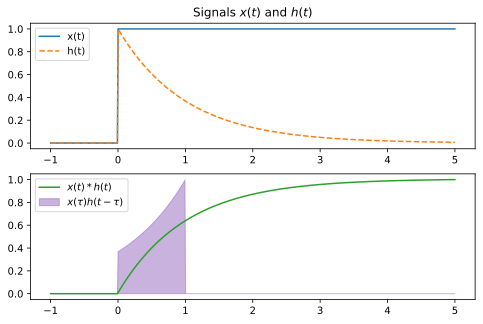
\includegraphics[width=.7\linewidth]{imgs/sig_conv/signals_conv}
    \caption{Illustration of the convolution operator between the Heaviside step function and a causal decreasing exponential.}
    \label{fig:convolution}
  \end{figure}
\end{warpprint}
%\begin{center}
  %\only<1>{ 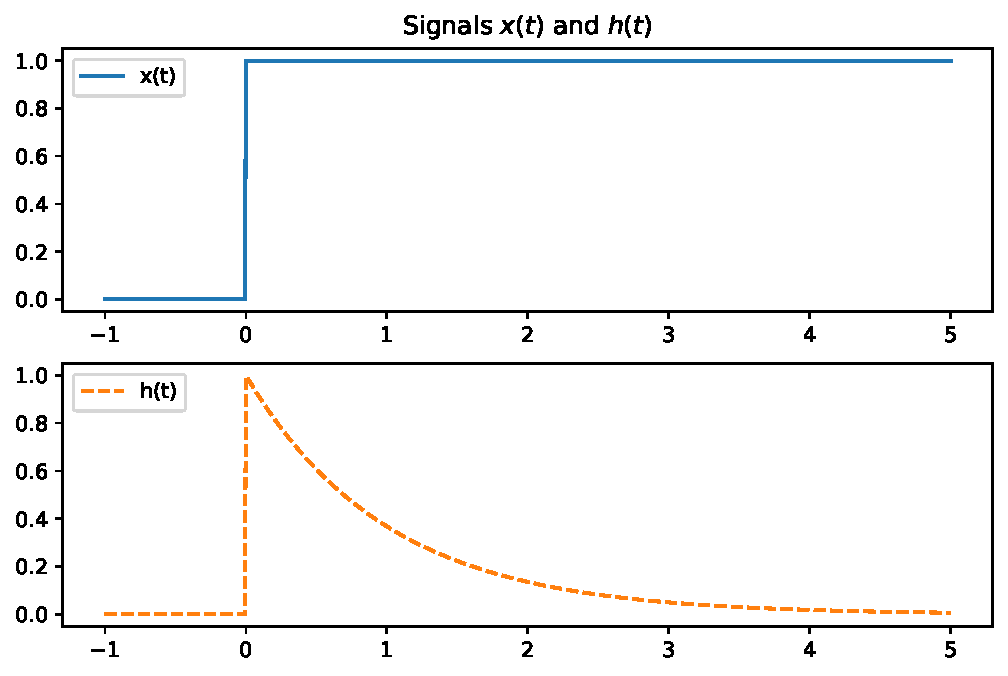
\includegraphics[width=.64\linewidth]{imgs/conv_demo/signals}}

 % \only<2>{ \inlineMovie{imgs/conv_demo/movie.mp4}{imgs/conv_demo/conv_000}{width=.64\linewidth}}
%\only<3>{ 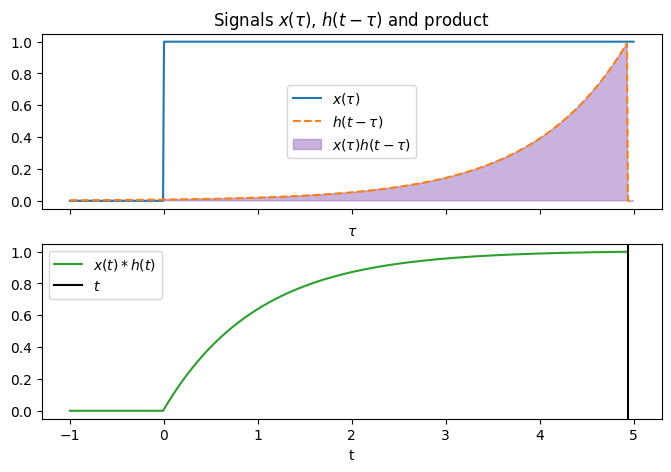
\includegraphics[width=.64\linewidth]{imgs/conv_demo/conv_098}}


\begin{itemize}
\item $x(t)=\Gamma(t)$ the Heaviside step function.
\item $h(t)=e^{-t}\Gamma(t)$ the positive part of the decreasing exponential.
\item $x(t)\star h(t)=(1-e^{-t})\Gamma(t)$
\end{itemize}

\subsection{Linear Time Invariant (LTI) systems}
\label{sec:lti_systems}



\begin{block}{Linear Time Invariant (LTI) system}\vspace{-1mm} \index{Linear
Time Invariant system}\index{LTI system}
  \begin{itemize}
  \item A system describes a relation between an input $x(t)$ and an output $y(t)$.
  \item Properties of LTI systems:\vspace{-1mm}
    \begin{itemize}
    \item Linearity \vspace{-3mm}
      $$\quad x_1(t)+ax_2(t)\rightarrow y_1(t)+ay_2(t)$$
    \item Time invariance\vspace{-3mm}
$$x(t-\tau)\rightarrow y(t-\tau)$$
    \end{itemize}
    \item A LTI system can most of the time be expressed as a convolution of the form:
    $$y(t)=x(t)\star h(t)$$
    where $h(t)$ is called the impulse response (the response of the system to an input $x(t)=\delta(t)$)
  \end{itemize}
\end{block}


\begin{exampleblock}{Examples}
\begin{itemize}
\item Passive electronic systems (resistor/capacitor/inductor) .
\item Newtonian mechanics, Fluid mechanics, Fourier Optics.
\end{itemize}
\end{exampleblock}



\begin{block}{Ordinary Differential Equation (ODE)} \index{Ordinary Differential Equation}
  The system is defined by a linear equation of the form:
  \begin{equation}
    \label{eq:edo}
    a_0y(t)+a_1\frac{dy(t)}{dt}+\dots+a_n\frac{d^ny(t)}{dt^n}=
    b_0x(t)+b_1\frac{dx(t)}{dt} +\dots+b_m\frac{d^mx(t)}{dt^m}
  \end{equation}
  
  \begin{itemize}
  \item ODE based system with linear relations are an important class of LTI systems.
  \item Also called homogeneous linear differential equation.
  %\item $\max(m,n)$ est l'ordre du système.
  %\item Également appelées équations différentielles linéaires à coefficients
  %constants.
  \item $n$ is the number of derivatives for $y(t)$ and $m$ for $x(t)$.
  \item $\max(m,n)$ is the order of the system.
  \item The output of the system can be computed from the input by solving Eq.
    \eqref{eq:edo}.
    \item Linearity and time invariance are obvious from equation.
  \end{itemize}
  
  \end{block}


\section{Discrete time and digital signals}
\label{sec:def_discrete_signal}

\subsection{Discrete time}

  \index{Discrete time!Definition}
\begin{block}{Notations}
  \begin{itemize}
      \item $x(t)$ with $t\in\R$ is the analog signal.
      \item $x_T(t)$ with $t\in\R$ is the sampled signal of period (T) but still continuous time:
      $$  x_T(t)=\sum_{n=-\infty}^\infty x(nT)\delta(t-nT) $$
      \item $x[n]$ with $n\in\mathbb{Z}$ is the discrete signal sampled with period $T$ such that:
      $$  x[n]= x(nT) $$
      \item Obviously one can recover $x_T(t)$ from $x[n]$ with
      $$  x_T(t)=\sum_{n=-\infty}^\infty x[n]\delta(t-nT) $$
      \item In order to simplify notations we will suppose $T=1$ in the following.
      \item In this course we suppose that $|x[n]|$ is bounded.
  \end{itemize}
\end{block}


\begin{center}
  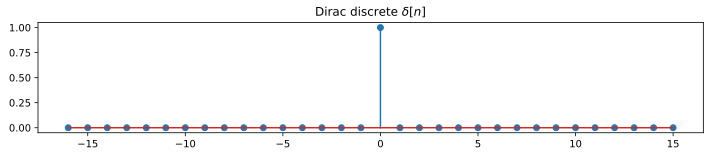
\includegraphics[width=.8\linewidth]{imgs/sig_conv/dirac_delta_discrete}
\end{center}\vspace{-5mm}

\index{Discrete time!Dirac Delta}\index{Dirac delta}
\begin{block}{Discrete dirac}
  We note the discrete dirac $\delta[n]$ defined as\vspace{-2mm}
  \begin{equation}
      \delta[n]=
      \begin{cases}
          1& \text{for } n=0\\
          0 & \text{else}
        \end{cases}
      \label{eq:discrete_dirac}
  \end{equation}\vspace{-5mm}
\end{block}

\begin{block}{Discrete signal}\index{Discrete time!Signal}
  Any discrete signal $x[n]$ can be decomposed as a sum of translated discrete diracs:\vspace{-1mm}
  \begin{equation}
      x[n]=\sum_{k=-\infty}^\infty x[k]\delta[n-k]
      \label{eq:discreet_signal_dirac}
  \end{equation}\vspace{-2mm}

  The discrete diracs are an orthogonal basis of $L_2(\mathbb{Z})$ of scalar product and corresponding norm  \vspace{-2mm}$$<x[n],h[n]>=\sum_{k=-\infty}^\infty x[k]h^*[k],\qquad \|x[n]\|^2=<x[n],x[n]>=\sum_{k=-\infty}^\infty |x[k]|^2.$$ 
\end{block}


\begin{block}{Convolution between discrete signals}\index{Discrete
time!Convolution}\index{Discrete convolution}\index{Digital filtering!Convolution}
  Let $x[n]$ and $h[n]$ two discrete signals. The convolution between them is expressed as:
  \begin{equation}
      x[n]\star h[n]= \sum_{k=-\infty}^\infty x[k]h[n-k]
      \label{eq:discrete_convolution}
  \end{equation}

\end{block}

\begin{block}{Digital filter properties}\index{Digital filtering!Properties}
  Let the discrete system/operator/filter $L$ described by its impulse response $h[n]$.
  \begin{itemize}
      \item \textbf{Causality} $L$ is causal if $h[n]=0,\ \forall n\leq 0$. $L$ is causal if 
   \begin{equation}
          h[n]=h[n]\Gamma[n],\qquad\text{where}\qquad     \Gamma[n]=
          \begin{cases}
              1& \text{for } n\geq 0\\
              0 & \text{else}
            \end{cases}
          \label{eq:causal_discrete}
      \end{equation}
      \item \textbf{Stability} A system is stable if the output of a bonded input is bounded. A necessary and sufficient condition is that
      \begin{equation}
          \sum_{n=-\infty}^\infty |h[n]|<\infty
          \label{eq:stable_system}
      \end{equation}
      
      
  \end{itemize}
  
\end{block}

\subsection{Finite signals}
\label{sec:finite}

\index{Finite signals}

\begin{center}
  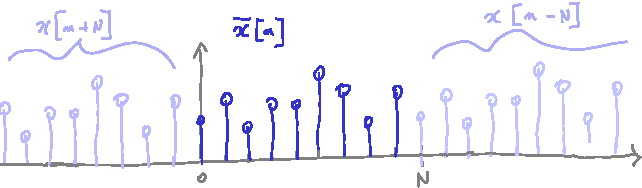
\includegraphics[width=.8\linewidth]{imgs/sig_conv/finite_discrete-crop.pdf}
\end{center}

\begin{block}{Finite discrete signals}\index{Discrete time!Finite Signal}
  \begin{itemize}
      \item Most of the theoretical results seen up to now correspond to signals $x[n]$ where $n\in\mathbb{Z}$.
      \item In practice recordings are only done for a finite amount of time resulting to only $N$ samples. 
      \item We defined $\tilde x[n]$ a finite signal of $N$ samples with $n\in \{0,\dots,N-1\}$.
      \item We use in the following the periodization of $\bar x[n]$
      $$ x[n] = \tilde x[n\mod N] $$
      where $\mod$ is the modulo operator.
  \end{itemize}
\end{block}

\begin{block}{Discrete convolution of finite signals}\index{Discrete time!Convolution}\index{Discrete convolution}
  The convolution between $\tilde x[n]$ and $\tilde h[n]$ both finite signals of $n$ samples can be expressed as:
  \begin{equation}
      \tilde y[n]=\tilde x[n]\star\tilde h[n] =  \sum_{p=-\infty}^{+\infty}
      \tilde x[p] \tilde h[n-p] 
      \label{eq:conv_finite}\vspace{-3mm}
  \end{equation}
  \begin{itemize}
      \item It requires values for the signals outside of the sampling widow. 
      \item One common approach consists in having $\tilde x[n]$ and $\tilde h[n]$ equal to $0$ outside the sampling interval. Other choices can be done (see next slides)
 %     \item In this case only the center sample is exact.
  \end{itemize}
\end{block}

\begin{block}{Circular convolution}\index{Discrete time!Circular convolution}\index{Circular convolution}
  When using the periodic version of the signals the circular convolution can be computed on a unique period of size $N$:
  \[
      x \ostar h [n] 
      = \sum_{p=0}^{N-1}
      x[p] h[n-p] .
      \] 
The circular convolution is rarely appropriate in real life images due to border effects.
 % Note that thanks to the 
\end{block}

\begin{block}{Vector representation and convolution
matrix}\vspace{-2mm}\index{Convolution matrix}
  \begin{itemize}
      \item Finite signal $x$ of $N$ samples can be represented as a vector $\x\in\mathbb{C}^N$.
      \item The convolution operator is linear and can be expressed as:\vspace{-1mm}
      $$ \y=\x\star\h= \C_\h \x $$
      Where\vspace{-1mm} $\C_\h\in \mathcal{M}_\mathbb{C}(N,N)$ is a convolution matrix parametrized by vector $\h$.
  \end{itemize} \vspace{-4mm}
\end{block} %\vspace{-5mm}

\begin{block}{Discrete convolution}\index{Discrete convolution}
  The convolution operator when the values outside the support are $0$ can be expressed as\vspace{-2mm}
  $$ \hspace{-3mm}\C_\h\hspace{-.5mm} =\hspace{-.5mm}\begin{bmatrix}
      h[0] & 0 & \cdots& 0\\
      h[1] & h[0] & \cdots& 0\\
      \vdots & \vdots & \ddots & \vdots\\
      h[N\hspace{-.5mm}-\hspace{-.5mm}1] & h[N\hspace{-.5mm}-\hspace{-.5mm}2 ] & \dots&  h[0]\\
      \vdots & \vdots & \ddots & \vdots\\
      0 & 0 &\cdots & h[N\hspace{-.5mm}-\hspace{-.5mm}1] 
  \end{bmatrix} $$
  where $\C_\h\in \mathcal{M}_\mathbb{C}(2*N-1,N)$ is a Toeplitz matrix.
\end{block}

\begin{block}{Circular convolution}\index{Circular convolution}
  The circular convolution operator can be expressed as
  $$ \C_\h =\begin{bmatrix}
      h[0] & h[N-1] & \cdots& h[1]\\
      h[1] & h[0] & \cdots& h[2]\\
      \vdots & \vdots & \ddots & \vdots\\
      h[N-1] & h[N-2 ] & \dots&  h[0]\\
  \end{bmatrix} $$
  where $\C_\h\in \mathcal{M}_\mathbb{C}(N,N)$ is a circulant Toeplitz matrix.
\end{block}

\begin{center}
  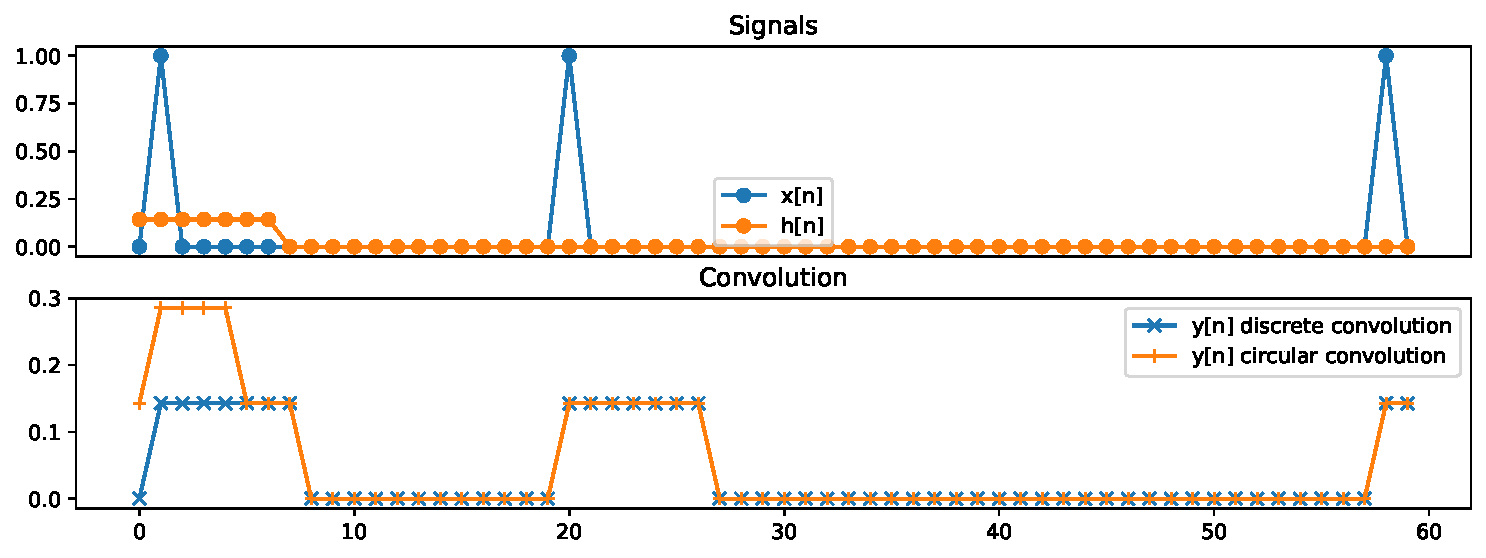
\includegraphics[width=.9\linewidth]{imgs/sig_conv/circ_conv_border.pdf}
\end{center}

\begin{itemize}
  \item Convolution between diracs $\tilde x[n]$ and a shape $h[n]$ will repeat the shape at the diracs position.
  \item A dirac at the end of the signal will cut the shape for discrete convolution where the outside of the sampling is $0$.
  \item With circular convolution the shape is repeated t the beginning of the signal.
  \item One can remove border effects by creating virtual periodic signal with zeros (zero padding, see fast convolution).
\end{itemize}



\begin{center}
  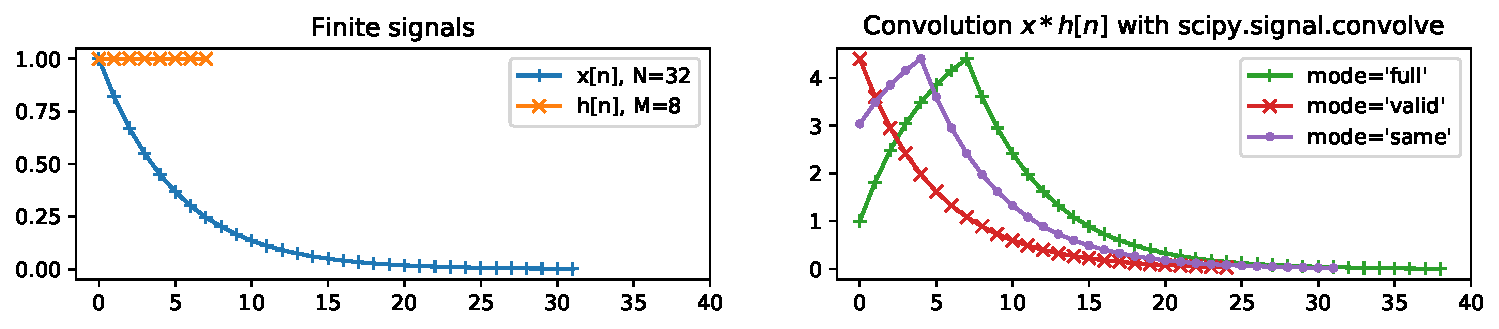
\includegraphics[width=1\linewidth]{imgs/sig_conv/conv_scipy_signal.pdf}
\end{center}\vspace{-2mm}

\begin{block}{The Scipy \incode{scipy.signal.convolve} function:}\vspace{-2mm}
  \begin{itemize} \index{Python!\incode{scipy.signal.convolve}}
      \item Convolution between two signals of support respectively $N$ and $M$ samples supposing that their values are $0$ outside of the support.
      \item The third parameter is \incode{mode} that change the size of the output : \vspace{-1mm}
      \begin{itemize}
          \item \incode{mode='full'} returns a signal of support $N+M-1$ (default).
          \item \incode{mode='valid'} returns a signal of support $|N-M|+1$ with only  the samples that do not rely on zeros padding of the larger signal.
          \item \incode{mode='same'} returns a signal of the same size as the first input.
      \end{itemize}
      \item Parameter \incode{method} allows to choose between \incode{'direct'} computation and \incode{'fft'} and selects the most efficient by default.
  \end{itemize}
  

  
\end{block}\vspace{-2mm}


\begin{center}
  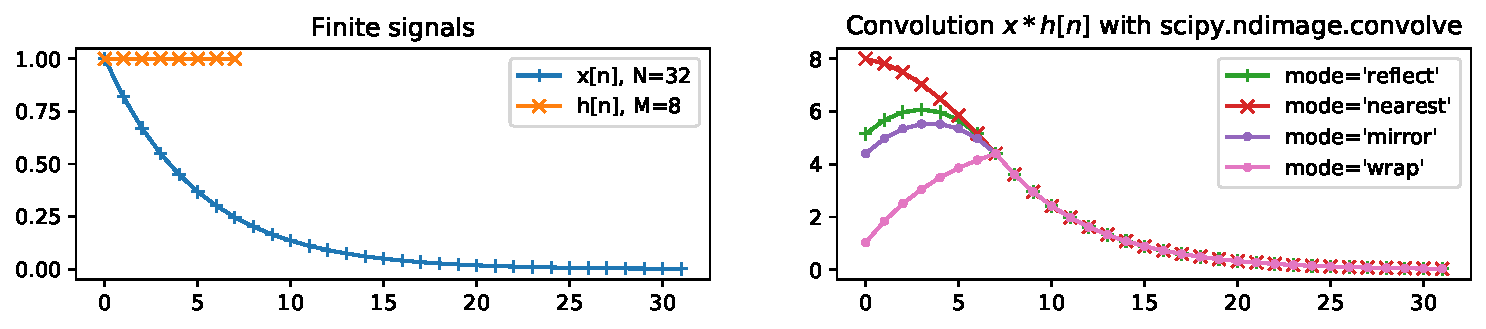
\includegraphics[width=1\linewidth]{imgs/sig_conv/conv_scipy_ndimage.pdf}

\end{center}\vspace{-2mm}

\begin{block}{The Scipy \incode{scipy.ndimage.convolve}  function:}\vspace{-2mm}
  \begin{itemize}\index{Python!\incode{scipy.ndimage.convolve}}
      \item Always return the same size as the first parameter by default.
      \item  The \incode{mode} parameter allows selecting the borders of a signal $x=(abcd)$:
      \begin{itemize}
          \item \incode{mode='reflect'} : $(d c b a | a b c d | d c b a)$ (default)
          \item  \incode{mode='constant'} : $(k k k k | a b c d | k k k k)$
          \item \incode{mode='nearest'} : $(a a a a | a b c d | d d d d)$
          \item \incode{mode='mirror'} : $(d c b | a b c d | c b a)$
          \item \incode{mode='wrap'} : $(a b c d | a b c d | a b c d)$ (circular convolution)
      \end{itemize}
      \item  Parameter \incode{origin} allows to select the origin of the filter $h$.
  \end{itemize}
  


\end{block}


\subsection{Quantization and storage}
\label{sec:}

\index{Quantization}

\section{Fundamental signal processing problems}
\label{sec:sp_prob}

\subsection{Filtering}

\index{Filtering}


\subsection{Deconvolution, unmixing and regression}

\index{Deconvolution}

\index{Inverse problem}


\subsection{Blind source separation and deconvolution}

\index{Blind source separation}



